\documentclass[t,aspectratio=169]{beamer}

\usepackage{soul}
\usepackage{tikz}
\usepackage{multicol}
%\usepackage{gensymb}
\usepackage[utf8]{inputenc}

\usetikzlibrary{arrows.meta,decorations.markings,decorations.pathreplacing,positioning}


\usepackage{hyperref}
\hypersetup{
    colorlinks=true,
    linkcolor=blue,
    filecolor=magenta,      
    urlcolor=cyan,
    pdftitle={(KTXFI1EBNF) Physics I. Practice},
}

% ----------------------------------------------------------------------------------------------------------------------------------------

\title{\includegraphics[width=45pt]{oepecsetlogo.png}\\(KTXFI1EBNF) Physics I. Practice}

\author{Dr.~Gábor FACSKÓ, PhD\\\tiny Assistant Professor / Senior Research Fellow\\\textit{facsko.gabor@uni-obuda.hu}}

\institute{\Tiny Óbuda University, Kandó Kálmán Faculty of Electrical Engineering, 1084 Budapest, Tavaszmező u. 17.\\Wigner Research Centre for Physics, Department of Space Physics and Space Technology, 1121 Budapest, Konkoly-Thege Miklós út 29–33.\\ \url{https://wigner.hu/~facsko.gabor}}

\date{May~4,~2026}

\logo{\includegraphics[height=0.9 true cm]{kekcsik.png}}

% ----------------------------------------------------------------------------------------------------------------------------------------

\begin{document}

\frame{\titlepage}

% ----------------------------------------------------------------------------------------------------------------------------------------

\begin{frame}
\frametitle{Current Updates and Announcements}
\begin{itemize}
\setlength{\parskip}{0pt}
\setlength{\itemsep}{4pt}
\item May 4, and go\dots
\item Homework No.~3 is now available tonight. The deadline is May 10, 2026 at midnight.
\item I promised a sample exam. I provided $\sim$100 questions on Moodle.
\item Today there is only practice of three different type of exercises. 
\end{itemize}
\end{frame}

% ----------------------------------------------------------------------------------------------------------------------------------------

\begin{frame}[fragile,squeeze,allowframebreaks]
\frametitle{Exercises}
\begin{itemize}
\setlength{\parskip}{0pt}
\setlength{\itemsep}{0pt}
\item \textbf{Thermodynamics I:} Temperature scales, thermal expansion, thermometers. State variables, ideal gas, state changes, ideal gas equation of state, Boyle’s law, Gay-Lussac’s laws, universal (combined) gas law, heat, specific heat, molar heat, heat capacity.
\item \textbf{Thermodynamics II:} Expansion work, internal energy, the first law of thermodynamics, forms of the first law in different state changes.
\item \textbf{Thermodynamics III:} Cyclic processes, Carnot cycle, Carnot’s theorem, reduced heat, entropy, the second law of thermodynamics.
\item \textbf{Thermodynamics IV:} Kinetic theory of gases, molecular thermodynamics. Distributions, distribution functions. Elementary statistics.
\item \textbf{Electrostatics I.:} Electric charge: Fundamental electrical phenomena, electric charge and matter, Coulomb’s law (force between two point charges, unit of electric charge, permittivity of vacuum).

\pagebreak
\item \textbf{Electrostatics II.:} The electric field: The electrostatic field (electric field strength, electric field lines). Determination of electric field strength. Gauss’s law (flux of the electric field). Electric field of a point charge.
\item \textbf{Electrostatics III.:} Electrostatic potential: Work of the electric field (work done in an electric field). Electric potential (electrostatic potential). Electric potential difference, voltage. Electric potential of charge systems at small and large distances. Electrostatic energy.
\item \textbf{Elements of physical or wave optics.} Branches of optics. Light interference, light diffraction, diffraction through a slit, optical grating, light polarization. Light as an electromagnetic wave: Poynting vector. Optical instruments.
\end{itemize}

\end{frame}

% ----------------------------------------------------------------------------------------------------------------------------------------

\begin{frame}[fragile,squeeze,allowframebreaks]
\frametitle{Oscillations and Waves}

\begin{enumerate}

\item  Given the displacement-time function of the oscillation:  
$$y(t) = 1.6 \sin(1.3t - 0.75)\,cm. $$ 
At $t=0\,s$, determine:
\begin{enumerate}
\item[a)] displacement,
\item[b)] velocity,
\item[c)] acceleration.
\end{enumerate}

\vskip -25 pt
\begin{columns}
  \begin{column}{0.3\linewidth}
    \vfill
\begin{center}
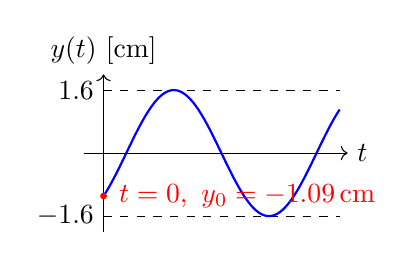
\begin{tikzpicture}[scale=0.5]
\draw[->] (-0.5,0) -- (6.2,0) node[right] {$t$};
\draw[->] (0,-2) -- (0,2) node[above] {$y(t)$ [cm]};

\draw[dashed] (0,1.6) -- (6,1.6);
\draw[dashed] (0,-1.6) -- (6,-1.6);
\node[left] at (0,1.6) {$1.6$};
\node[left] at (0,-1.6) {$-1.6$};

\draw[thick,blue,domain=0:6,samples=200]
plot(\x,{1.6*sin((1.3*\x-0.75) r)});

\filldraw[red] (0,{1.6*sin((-0.75) r)}) circle (2pt);
\node[right,red] at (0.15,{1.6*sin((-0.75) r)})
{$t=0,\ y_0=-1.09\,\mathrm{cm}$};

%\node[align=left] at (3,-2.6) {$y(t)=1.6\sin(1.3t-0.75)\,\mathrm{cm}$, $y(0)=-1.09\,\mathrm{cm}$, $v(0)=1.52\,\mathrm{cm/s}$, $a(0)=1.84\,\mathrm{cm/s^2}$};
\end{tikzpicture}
\end{center}
\end{column}
\begin{column}{0.7\linewidth}
Convert amplitude: $1.6\ \mathrm{cm} = 0.016\ \mathrm{m}$  
\begin{enumerate}
\item[a)] $y(0) = 0.016\,\mathrm{m}\sin(-0.75) = -0.0109\ \mathrm{m}$  
\item[b)] Velocity: $v(t) = \frac{dy(t)}{dt} = 0.016\,\mathrm{m} \cdot 1.3\,\mathrm{s^{-1}}\cos(1.3t - 0.75)$  
$v(0) = 0.0208\,\mathrm{m/s}\cos(-0.75) = 0.0152\ \mathrm{m/s}$  
\item[c)] Acceleration: $a(t) =  \frac{dv(t)}{dt} = -0.016\,\mathrm{m} \cdot (1.3\mathrm{s^{-1}})^2 \sin(1.3\,\mathrm{s^{-1}}\,t - 0.75) $  
  $a(0) = 0.0184\ \mathrm{m/s^2}$
\end{enumerate}
\end{column}
\end{columns}

\pagebreak

\item  Given the sum of two one-directional oscillation as the following $x(t) = 3\sin(\omega t) + 4\cos(\omega t).$ This describes the displacement - time function of the oscillation, where t represents time, $\omega$ denotes the circular frequency of the oscillation, and $\omega$ is a constant.
\begin{enumerate}
  \item[a)] Prove that the above x(t) oscillation, given by the displacement-time function, performs simple harmonic motion.
  \item[b)] What is the value of the resultant oscillation given by the above displacement-time function?
\end{enumerate}

\begin{enumerate}
\item[a)] 
First, let’s take the first and second time derivatives of $x\left(t\right)$!
\begin{eqnarray*}
\frac{dx\left(t\right)}{dt}&=&\dot{x}(t) = 3\omega \cos(\omega t) - 4\omega \sin(\omega t)\\
  \frac{d^{2}x\left(t\right)}{dt^{2}}&=&\ddot{x}(t) = -3\omega^2 \sin(\omega t) - 4\omega^2 \cos(\omega t)
\end{eqnarray*}
After that, let’s form the ratio of $\frac{\ddot{x}\left(t\right)}{x\left(t\right)}$
\begin{eqnarray*}
  \frac{\ddot{x}(t)}{x(t)} &=& \frac{-3\omega^2 \sin(\omega t) - 4\omega^2 \cos(\omega t)}{3 \cos(\omega t) - 4 \sin(\omega t)} =  \frac{\omega^{2}\left[-3 \sin(\omega t) - 4 \cos(\omega t)\right]}{3 \cos(\omega t) - 4 \sin(\omega t)} = -\omega^2 \\
\frac{\ddot{x}(t)}{x(t)} &=& -\omega^2 \\
\ddot{x}(t) &=& -\omega^2 x(t)
\end{eqnarray*}
where $-\omega^{2}$ is constant. This is precisely the equation of the harmonic motion. Thus, the oscillation is harmonic.

\item[b)] To calculate the amplitude, we use the amplitude formula:
  $$A = \sqrt{A^{2}_{1} + A^{2}_{2} + 2 \cdot A_{1} \cdot A_{2} \cdot \cos\left(\varphi_{1} - \varphi_{2}\right)}$$

\pagebreak
\begin{columns}
  \begin{column}{0.4\linewidth}
    \begin{center}
\begin{tikzpicture}[scale=0.7]
\draw[->] (-0.5,0) -- (5.8,0) node[below] {$\cos(\omega t)$};
\draw[->] (0,-0.5) -- (0,4.8) node[above] {$\sin(\omega t)$};

\draw[thick,blue,->] (0,0) -- (4,0) node[midway,below] {$4$};
\draw[thick,red,->] (4,0) -- (4,3) node[midway,right] {$3$};

\draw[thick,purple,->] (0,0) -- (4,3)
node[midway,above left] {$A=5$};

\draw[dashed] (4,0) -- (4,3);
\draw[dashed] (0,3) -- (4,3);

\node[left] at (0,3) {$3$};
\node[below] at (4,0) {$4$};

\draw (1,0) arc[start angle=0,end angle=36.87,radius=1];
\node at (1.25,0.35) {$\varphi$};

\node[align=left] at (3,-1.1)
{$\tan\varphi=\dfrac{3}{4}$\\
$\varphi=36.87^\circ$};

\node[align=left] at (3,4.3)
{$x(t)=3\sin(\omega t)+4\cos(\omega t)$\\
$x(t)=5\sin(\omega t+\varphi)$};
\end{tikzpicture}
\end{center}
\end{column}
\begin{column}{0.7\linewidth}
Calculating the phase difference:
$x\left(t\right) = 3 \cdot \sin\left(\omega t\right) + 4 \cdot \cos\left(\omega t\right) = 3 \cdot \sin\left(\omega t\right) + 4 \cdot \sin\left(\omega t + \frac{\pi}{2} \right)$
$\cos\left(\alpha\right) =\sin\left(\alpha + \frac{\pi}{2}\right)$

The phase difference: $\varphi_{1} = \omega t$, $\varphi_{2} = \omega t + \frac{\pi}{2}$.
$$  \varphi_{1} - \varphi_{2} = -\frac{\pi}{2}$$
$A = \sqrt{A^{2}_{1} + A^{2}_{2} + 2 \cdot A_{1} \cdot A_{2} \cdot \cos\left(\varphi_{1} - \varphi_{2}\right)}=\sqrt{3^2+4^2+2\cdot 3\cdot 4 \cos\left(-\frac{\pi}{2}\right)}$

Therefore, the amplitude is A = 5.
\end{column}
\end{columns}

\end{enumerate}

\pagebreak

\item Consider three one-directional oscillations with equal frequencies, whose amplitudes and initial phases are given as follows:
\begin{eqnarray*}
A_1 = 7 \cdot 10^{-3},\mathrm{m}&,& \varphi_1 = \pi/3 \\
A_2 = 5 \cdot 10^{-3}\,\mathrm{m}&,& \varphi_2 = 5\pi/6 \\
A_3 = 2 \cdot 10^{-3}\,\mathrm{m}&,& \varphi_3 = 23\pi/18
\end{eqnarray*}
Let’s combine these three oscillations. Calculate the amplitude and initial phase of the resultant vibration!

The amplitude of the resultant oscillation - sum of oscillations - can be calculated as follows:

$$x(t)=A\sin(\omega t+\varphi)$$

\pagebreak
\begin{columns}
\begin{column}{0.25\linewidth}
\begin{center}
  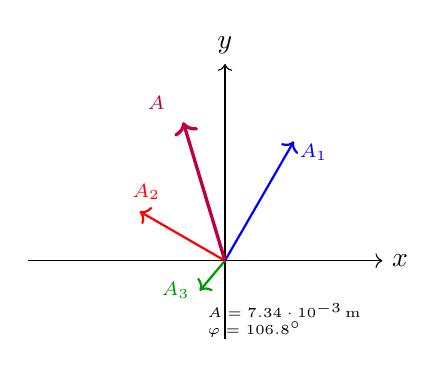
\begin{tikzpicture}[scale=250]
\draw[->] (-0.010,0) -- (0.008,0) node[right] {$x$};
\draw[->] (0,-0.004) -- (0,0.010) node[above] {$y$};

% vectors
\draw[thick,blue,->]
(0,0) -- ({0.007*cos(60)},{0.007*sin(60)});

\draw[thick,red,->]
(0,0) -- ({0.005*cos(150)},{0.005*sin(150)});

\draw[thick,green!60!black,->]
(0,0) -- ({0.002*cos(230)},{0.002*sin(230)});

% resultant
\draw[very thick,purple,->]
(0,0) -- (-0.00212,0.00703);

% labels
\node[blue,font=\scriptsize] at (0.0045,0.0055) {$A_1$};
\node[red,font=\scriptsize] at (-0.004,0.0035) {$A_2$};
\node[green!60!black,font=\scriptsize] at (-0.0025,-0.0015) {$A_3$};
\node[purple,font=\scriptsize] at (-0.0035,0.008) {$A$};

\node[align=left,font=\tiny] at (0.003,-0.003)
{$A=7.34\cdot10^{-3}\,\mathrm{m}$\\
$\varphi=106.8^\circ$};
\end{tikzpicture}
\end{center}
\end{column}
\begin{column}{0.7\linewidth}
Using vector addition:
\begin{eqnarray*}
A\sin\varphi &=& \sum_i A_i\sin\varphi_i \\
A\cos\varphi &=& \sum_i A_i\cos\varphi_i
\end{eqnarray*}
Hence,
\begin{eqnarray*}
A\sin\varphi&=&7\cdot10^{-3}\sin\frac{\pi}{3}+5\cdot10^{-3}\sin\frac{5\pi}{6}+2\cdot10^{-3}\sin\frac{23\pi}{18} \\
A\cos\varphi&=&7\cdot10^{-3}\cos\frac{\pi}{3}+5\cdot10^{-3}\cos\frac{5\pi}{6}+2\cdot10^{-3}\cos\frac{23\pi}{18}
\end{eqnarray*}

\end{column}
\end{columns}


\pagebreak
Numerically:
\begin{eqnarray*}
A\sin\varphi&=&0.007 \\
A\cos\varphi&=&-0.002
\end{eqnarray*}
Dividing:
$$\tan\varphi=\frac{A\sin\varphi}{A\cos\varphi}=\frac{0.007}{-0.002}=-3.5$$
Thus:
$$\varphi\approx105.945^\circ$$
or
$$\varphi\approx1.85\ \mathrm{rad}$$

\pagebreak
Using:
$$A\sin\varphi=0.007$$
we obtain:
$$A\approx7.3\cdot10^{-3}\ \mathrm{m}$$

\pagebreak

\item  Calculate and determine the curve described by the resultant of the perpendicular vibrations given by the equations:
\begin{eqnarray*}
x(t) &=& x_0 \cos(\omega t),\\  
y(t) &=& y_0 \cos(2\omega t).  
\end{eqnarray*}

\begin{columns}
\begin{column}{0.3\linewidth}
 \begin{center}
 \vskip -70 pt
  \begin{tikzpicture}[scale=1.5]
\draw[->] (-1.4,0) -- (1.4,0) node[right] {$x$};
\draw[->] (0,-1.3) -- (0,1.3) node[above] {$y$};

% curve: y = 2x^2 - 1, normalized
\draw[thick,blue,domain=-1:1,samples=100]
plot(\x,{2*\x*\x-1});

% auxiliary dashed lines
\draw[dashed] (-1,-1.1) -- (-1,1.1);
\draw[dashed] (1,-1.1) -- (1,1.1);
\draw[dashed] (-1.1,1) -- (1.1,1);
\draw[dashed] (-1.1,-1) -- (1.1,-1);

\node[below] at (-1,0) {$-x_0$};
\node[below] at (1,0) {$x_0$};
\node[left] at (0,1) {$y_0$};
\node[left] at (0,-1) {$-y_0$};

\node[blue] at (-0.6,1.6) {$y=y_0\left(2\dfrac{x^2}{x_0^2}-1\right)$};

\filldraw[red] (0,-1) circle (1.2pt);
\node[below right,red] at (0,-1) {$(0,-y_0)$};

\filldraw[red] (-1,1) circle (1.2pt);
\filldraw[red] (1,1) circle (1.2pt);
\end{tikzpicture}
\end{center}
\vfill
\end{column}
\begin{column}{0.7\linewidth}
The perpendicular oscillations are given by
\begin{eqnarray*}
x(t)&=&x_0\cos(\omega t) \\
y(t)&=&y_0\cos(2\omega t).
\end{eqnarray*}
\vskip -10 pt
First, express \(\cos(\omega t)\) from the first equation:
$$\cos(\omega t)=\frac{x}{x_0}.$$
\vfill
\end{column}
\end{columns}

\pagebreak
Next, use the trigonometric identity
$$\cos(2\alpha)=\cos^{2}\alpha-\sin^{2}\alpha=\cos^{2}\alpha+\left(\cos^{2}\alpha+\sin^{2}\alpha\right)-\sin^{2}\alpha-1=2\cos^2\alpha-1,$$
where $\sin^{2}\alpha+\cos^{2}\alpha=1$

Applying this identity to the second equation:
$$y=y_0\left(2\cos^2(\omega t)-1\right).$$
Substitute
$$\cos(\omega t)=\frac{x}{x_0}$$
into the equation:
\vskip -25 pt
$$y=y_0\left(2\left(\frac{x}{x_0}\right)^2-1\right).$$

\pagebreak
Therefore, the equation of the resultant curve is
$$\boxed{y=y_0\left(2\frac{x^2}{x_0^2}-1\right)}$$
which is the equation of a parabola.

\pagebreak

\item Let $f(\omega t \pm kx + \varphi)$ be a function whose argument is at least twice differentiable, continuous, and arbitrary, where $\omega$: constant circular frequency, k : wavenumber (constant), $\varphi$ initial phase (constant), t : time, x spatial coordinate. Prove that the function f described above is a solution to the one-dimensional wave equation.

  \begin{center}
    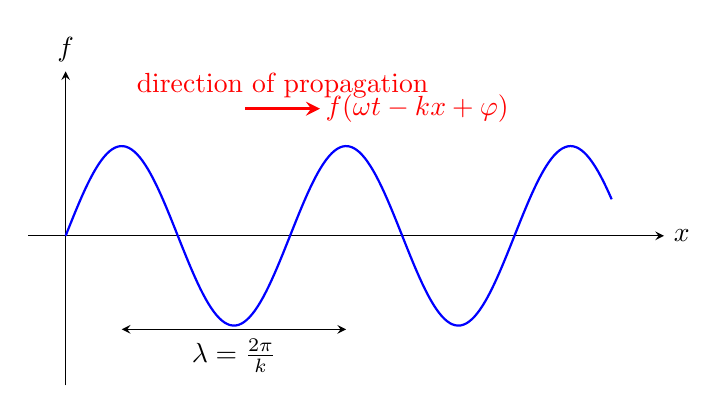
\begin{tikzpicture}[scale=0.95, >=stealth]
  % Axes
  \draw[->] (-0.5,0) -- (8,0) node[right] {$x$};
  \draw[->] (0,-2) -- (0,2.2) node[above] {$f$};

  % Wave profile
  \draw[thick, blue, domain=0:7.3, samples=200]
    plot (\x,{1.2*sin(120*\x)});

  % Right-moving label
  \draw[->, very thick, red] (2.4,1.7) -- (3.4,1.7)
    node[midway, above] {direction of propagation};
  \node[red] at (4.7,1.7) {$f(\omega t-kx+\varphi)$};

  % Phase argument box
%  \node[draw, rounded corners, align=center, fill=white] at (4,-1.55)
%  {
%    $\xi=\omega t \pm kx+\varphi$\\[2pt]
%    $f=f(\xi)$
%  };

  % Wave equation
% \node[draw, rounded corners, fill=white] at (4,2.25)
%  {
%    $\displaystyle \frac{\partial^2 f}{\partial t^2}
%    = v^2 \frac{\partial^2 f}{\partial x^2},
%    \qquad v=\frac{\omega}{k}$
%  };

  % Wavelength indication
  \draw[<->] (0.75,-1.25) -- (3.75,-1.25)
    node[midway, below] {$\lambda=\frac{2\pi}{k}$};

\end{tikzpicture}
  \end{center}


The one-dimensional wave equation is
$$\frac{\partial^{2}\psi}{\partial t^2}=c^2\frac{\partial^{2}\psi}{\partial x^{2}},$$
where c  is a constant, the wave velocity.

Let $\psi=f(\omega t\pm kx+\phi)$. Take the derivatives. Time derivatives:
\begin{eqnarray*}
\frac{\partial f}{\partial t}&=&\omega f'(\omega t\pm kx+\phi)\\
\frac{\partial^{2}f}{\partial t^2}&=&\omega^2 f''(\omega t\pm kx+\phi)
\end{eqnarray*}

\pagebreak
Spatial derivatives:
\vskip -10 pt
\begin{eqnarray*}
\frac{\partial f}{\partial x}&=&\pm k f'(\omega t\pm kx+\phi) \\
\frac{\partial^{2}f}{\partial x^2}&=&k^2 f''(\omega t\pm kx+\phi)
\end{eqnarray*}
 \vskip -5 pt 
 Substituting into the wave equation:
 \vskip -10 pt
$$\omega^2 f''(\omega t\pm kx+\phi)=c^2 k^2 f''(\omega t\pm kx+\phi)$$
\vskip -5 pt
Using the $\omega=kc$, $\omega^2=k^2c^2$ dispersion relations,
\vskip -10 pt
$$\omega^2 f''(\omega t\pm kx+\phi)=\omega^2 f''(\omega t\pm kx+\phi)$$

Hence both sides are identical, proving the statement.

Wave speed: $v = \frac{\omega}{k}\ \mathrm{[m/s]}$  

\pagebreak

\item The displacement of a wave as a function of time is given by $$y(x,t) = 0.27 \sin(12x - 500t)\,mm,$$ where x is in meters and t is given in seconds. Determine at the point x = 0.2 meters in the case of a transverse wave:
\begin{enumerate}
\item[a)] its velocity,
\item[b)] its acceleration!
\item[c)] What is the displacement of the point at t = 4s seconds?
\end{enumerate}


\begin{center}
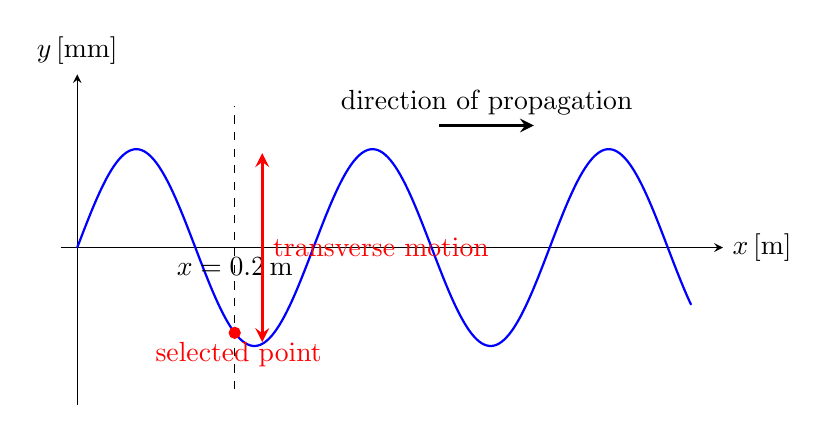
\begin{tikzpicture}[scale=1.0, >=stealth]
  % Axes
  \draw[->] (-0.2,0) -- (8.2,0) node[right] {$x\,[\mathrm{m}]$};
  \draw[->] (0,-2.0) -- (0,2.2) node[above] {$y\,[\mathrm{mm}]$};

  % Wave
  \draw[thick, blue, domain=0:7.8, samples=250]
    plot (\x,{1.25*sin(120*\x)});

  % Mark x = 0.2 m
  \draw[dashed] (2.0,-1.8) -- (2.0,1.8);
  \filldraw[red] (2.0,{1.25*sin(120*2.0)}) circle (2pt);

  \node[below] at (2.0,0) {$x=0.2\,\mathrm{m}$};
  \node[red, below] at (2.05,{1.25*sin(120*2.0)})
    {selected point};

  % Transverse motion arrow
  \draw[<->, very thick, red] (2.35,-1.2) -- (2.35,1.2)
    node[midway, right] {transverse motion};

  % Propagation direction
  \draw[->, very thick] (4.6,1.55) -- (5.8,1.55)
    node[midway, above] {direction of propagation};

  % Formula box
%  \node[draw, rounded corners, fill=white, align=center] at (4.5,-1.65)
%  {
%    $\displaystyle y(x,t)=0.27\sin(12x-500t)\,\mathrm{mm}$\\[2pt]
%    $\displaystyle A=0.27\,\mathrm{mm},\quad k=12\,\mathrm{m^{-1}},\quad \omega=500\,\mathrm{s^{-1}}$
%  };

  % Evaluation box
%  \node[draw, rounded corners, fill=white, align=center] at (5.0,2.05)
%  {
%    at $\displaystyle x=0.2\,\mathrm{m}$:\\[2pt]
%    $\displaystyle y(t)=0.27\sin(2.4-500t)\,\mathrm{mm}$
%  };
\end{tikzpicture}  
\end{center}

\begin{enumerate}
\item[a)] Velocity is $v=\frac{\partial y}{\partial t}$, 
\vskip -20pt
$$v=-0.27\cdot500\cos(12\,\mathrm{m^{-1}}x-500\,\mathrm{s^{-1}}t)\ \frac{\mathrm{mm}}{\mathrm{s}}$$

At \(x=0.2\,\mathrm{m}\):
\vskip -20pt
$$v=-0.135\cos(2.4-500\,\mathrm{s^{-1}}t)\ \frac{\mathrm{m}}{\mathrm{s}}$$

\item[b)] Acceleration is $a=\frac{\partial v}{\partial t}$, therefore, 
\vskip -10pt  
$$a=-0.135 \cdot 500 \cdot \sin(2.4 - 500\,s^{-1}t)\mathrm{m/s^2}=-67.5\sin(2.4-500\,\mathrm{s^{-1}}t)\ \frac{\mathrm{m}}{\mathrm{s}^2}$$

\item[c)] Displacement of the point at t = 4s:
\vskip -10pt 
$$y=0.27\cdot 10^{-3}\mathrm{m}\sin(12\,\mathrm{m^{-1}}\cdot0.2\,\mathrm{m}-500\,\mathrm{s^{-1}}\cdot4\,\mathrm{s})\approx0.118\ \mathrm{mm}$$

Convert amplitude: $0.27\ \mathrm{mm} = 2.7 \cdot 10^{-4}\ \mathrm{m}$  

\end{enumerate}

\end{enumerate}

\end{frame}

% ----------------------------------------------------------------------------------------------------------------------------------------

\begin{frame}[fragile,squeeze,allowframebreaks]
\frametitle{Rigid Bodies}

\begin{enumerate}

\item According to measurements, the position (in meters) of a body with a mass of 300\,g along the x-axis is given by the following function: $$x(t) = -t^2 + 7.5 t^3,$$ where t represents the time in seconds. Determine the resultant force acting on the body as a function of time! What is the magnitude of the resultant force at t=5\,s? 

  \begin{center}
\vskip -15 pt
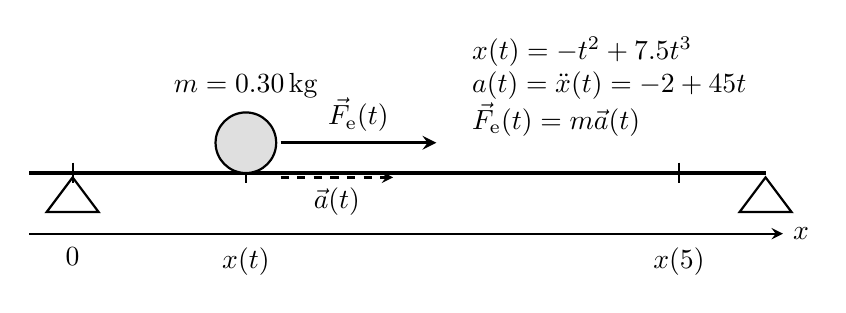
\begin{tikzpicture}[scale=1.1, >=stealth]

% rod / x-axis
\draw[very thick] (-0.5,0) -- (8,0);
\draw[->, thick] (-0.5,-0.7) -- (8.2,-0.7) node[right] {$x$};

% ticks
\foreach \x/\lab in {0/0,2/{$x(t)$},7/{$x(5)$}}
{
  \draw[thick] (\x,0.12) -- (\x,-0.12);
  \node[below] at (\x,-0.75) {\lab};
}

% body on rod
\draw[fill=gray!25, thick] (2,0.35) circle (0.35);
\node[above=0.45cm] at (2,0.35) {$m=0.30\,\mathrm{kg}$};

% resultant force arrow
\draw[->, very thick] (2.4,0.35) -- (4.2,0.35)
  node[midway, above] {$\vec F_\mathrm{e}(t)$};

% acceleration arrow
\draw[->, thick, dashed] (2.4,-0.05) -- (3.7,-0.05)
  node[midway, below] {$\vec a(t)$};

% label formulas
\node[align=left, right] at (4.5,1.0) {
  $x(t)=-t^2+7.5t^3$\\
  $a(t)=\ddot x(t)=-2+45t$\\
  $\vec F_\mathrm{e}(t)=m\vec a(t)$
};

% value at t=5
%\node[draw, rounded corners, align=center, fill=gray!10] at (6.5,0.8) {
%  $t=5\,\mathrm{s}$\\
%  $F_\mathrm{e}=66.9\,\mathrm{N}$
%};

% supports / stylized rod holder
\draw[thick] (0,-0.05) -- (-0.3,-0.45) -- (0.3,-0.45) -- cycle;
\draw[thick] (8,-0.05) -- (7.7,-0.45) -- (8.3,-0.45) -- cycle;

\end{tikzpicture}
\end{center}

\pagebreak

We know that $v(t) = \frac{dx(t)}{dt}$, $a(t) = \frac{dv(t)}{dt} = \frac{d^{2}x(t)}{dt^{2}}$, and $F (t) = m \cdot a(t)$. Furthermore, $m=300\,\mathrm{g}=0.300\,\mathrm{kg}$, $
x(t)=-t^2+7.5t^3\,\mathrm{m}$.

\begin{eqnarray*}
v(t)=\frac{dx(t)}{dt}=\frac{d}{dt}\left(-t^2+7.5t^3\right)&=&-2t+22.5t^2\,\mathrm{\frac{m}{s}},\\
a(t)=\frac{dv(t)}{dt}=\frac{d^2x(t)}{dt^2}&=&-2+45t\,\mathrm{\frac{m}{s^2}},\\
F_{\mathrm{e}}(t)=m\,a(t)&=&0.300\,\mathrm{kg}\cdot\left(-2+45t\right)\,\mathrm{\frac{m}{s^2}}=-0.6+13.5t\,\mathrm{N},\\
F_{\mathrm{e}}(5\,\mathrm{s})&=&-0.6+13.5\cdot5\,\mathrm{N},\\
F_{\mathrm{e}}(5\,\mathrm{s})&=&66.9\,\mathrm{N}.
\end{eqnarray*}

\pagebreak

\item A mass of 20 kg moves with a constant velocity at 12\,m/s. At some moment, we start to apply a force opposite to the direction of motion, which is not constant but increases steadily from zero at a rate of 40\,N/s . How much time elapses from the beginning of the force’s effect until the body comes to a complete stop (decelerates)?
A $20\ \mathrm{kg}$ mass moves with velocity $12\ \mathrm{m/s}$.  

\begin{center}
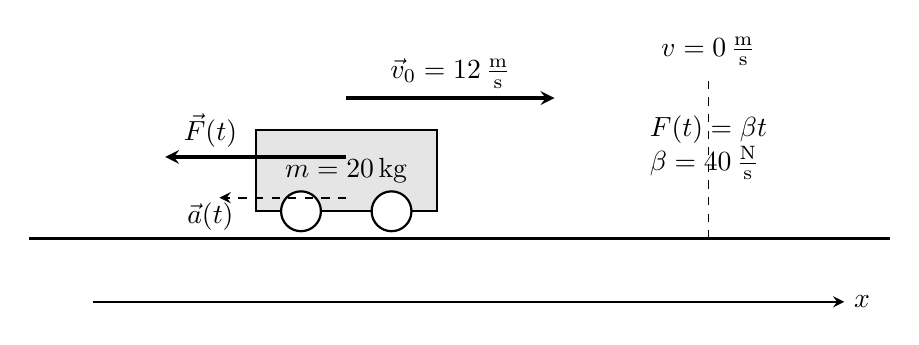
\begin{tikzpicture}[scale=1.15,>=stealth]

% ground
\draw[very thick] (-0.5,0) -- (9,0);

% cart
\draw[fill=gray!20,thick] (2,0.3) rectangle (4,1.2);

% wheels
\draw[thick,fill=white] (2.5,0.3) circle (0.22);
\draw[thick,fill=white] (3.5,0.3) circle (0.22);

% mass label
\node at (3,0.75) {$m=20\,\mathrm{kg}$};

% velocity arrow
\draw[->,very thick] (3,1.55) -- (5.3,1.55);
\node[above] at (4.15,1.55) {$\vec v_0=12\,\mathrm{\frac{m}{s}}$};

% braking force
\draw[->,very thick] (3,0.9) -- (1,0.9);
\node[above] at (1.5,0.9) {$\vec F(t)$};

% text about force
\node[align=left] at (7,1.0) {
$F(t)=\beta t$   \\
$\beta=40\,\mathrm{\frac{N}{s}}$
};

% acceleration arrow
\draw[->,thick,dashed] (3,0.45) -- (1.6,0.45);
\node[below] at (1.5,0.5) {$\vec a(t)$};

% stopping point
\draw[dashed] (7,0) -- (7,1.8);
\node[above] at (7,1.8) {$v=0\,\mathrm{\frac{m}{s}}$};

% motion direction
\draw[->,thick] (0.2,-0.7) -- (8.5,-0.7);
\node[right] at (8.5,-0.7) {$x$};

% time label
%\node[draw,rounded corners,fill=gray!10,align=center] at (7,0.9) {
%$t=\tau$
%$\tau=\sqrt{\frac{2mv_0}{\beta}}$
%};

\end{tikzpicture}
\end{center} 

The force can be expressed in the following form:

$$F = \beta t,$$

where $\beta = 40\,\mathrm{N/s}.$

According to Newton’s second law:

$$F = ma \Rightarrow a = \frac{F}{m}. $$

Substituting the expression for the force:

$$a = \frac{F}{m} = -\frac{\beta t}{m}. $$

\pagebreak
Therefore,

$$a = -\frac{\beta}{m} t,$$

and since

$$a = \frac{dv}{dt},$$

we obtain

$$\frac{dv}{dt} = -\frac{\beta}{m} t. $$

\pagebreak
Integrating both sides:

$$\int \frac{dv}{dt} \, dt = \int -\frac{\beta}{m} t \, dt$$

which gives

$$v = -\frac{\beta}{m} \int t \, dt = -\frac{\beta}{m} \cdot \frac{t^2}{2} + C. $$

Hence,

$$v = -\frac{\beta}{2m} t^2 + C. $$

\pagebreak
The integration constant is the initial velocity: $$C = v_0,$$where $v_0 = 12\,\mathrm{m/s}$ at $t = 0\,\mathrm{s}$ (beginning of the force action). Therefore,

$$v = v_0 - \frac{\beta}{2m} t^2. $$

When the object comes to a stop,$v = 0\,\mathrm{m/s}.$

Let the stopping time be denoted by $\tau$. Then:

$$0\,\mathrm{m/s} = v_0 - \frac{\beta}{2m} \tau^2$$

\pagebreak
hence,

$$\tau = \sqrt{\frac{2mv_0}{\beta}}. $$

Substituting the numerical values:

$$\tau = \sqrt{\frac{2mv_0}{\beta}}= \sqrt{\frac{2 \cdot 20\,\mathrm{kg} \cdot 12\,\mathrm{m/s}}{40\,\mathrm{N/s}}} = 3.5\,\mathrm{s}. $$

\pagebreak
\item A point-like object is subjected to a force in the x direction: $$F(x) = (3 + 0.5\,x)\,\mathrm{N}.$$ Determine the work done by the force as the mass point moves from x=0\,m to x=4\,m.

\begin{columns}
\begin{column}{0.5\linewidth}
\begin{center}
\vskip -30 pt
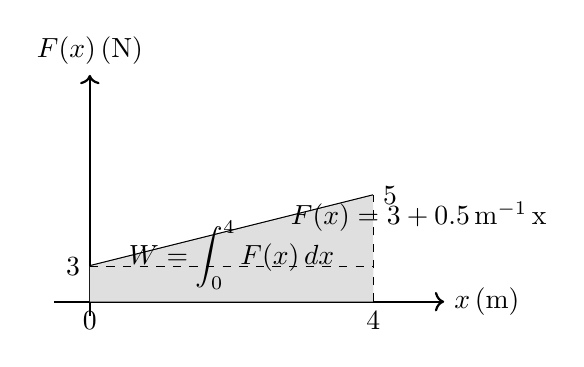
\begin{tikzpicture}[scale=0.9]

% axes
\draw[->, thick] (-0.5,0) -- (5,0) node[right] {$x\,(\mathrm{m})$};
\draw[->, thick] (0,-0.2) -- (0,3.2) node[above] {$F(x)\,(\mathrm{N})$};

% force function
\draw[thick, domain=0:4, samples=100] plot (\x,{0.5 + 0.25*\x});

% shaded area
\fill[gray!25, domain=0:4, samples=100]
  (0,0) -- plot (\x,{0.5 + 0.25*\x}) -- (4,0) -- cycle;

% boundary lines
\draw[dashed] (4,0) -- (4,1.5);
\draw[dashed] (0,0.5) -- (4,0.5);

% labels
\node[left] at (0,0.5) {$3$};
\node[right] at (4,1.5) {$5$};
\node[below] at (0,0) {$0$};
\node[below] at (4,0) {$4$};

\node at (2,0.65) {$W=\displaystyle\int_0^4 F(x)\,dx$};
\node[right] at (2.7,1.2) {$F(x)=3+0.5\,\mathrm{m^{-1}\,x}$};

\end{tikzpicture}
\end{center}
\vfill
\end{column}
\begin{column}{0.5\linewidth}
$W= \int_{g} \vec{F}  d\vec{s} = \int_0^4 (3 + 0.5\,x)\,dx\,\mathrm{J} = \left[ 3\,x + 0.25\,x^{2} \right]_0^4 \,\mathrm{J}= 12\,\mathrm{J} + 4\,\mathrm{J} = 16\,\mathrm{J}$
\end{column}
\end{columns}
  
\pagebreak

\item A 0.2\,kg mass stone slides without initial velocity from the top edge of a frictionless roof as depicted in the figure. $\alpha=40^{\circ}$ , g=10\,m/$s^{2}$ , h1=3\,m, h2=15\,m
\begin{enumerate}
\item[a)] What will be the magnitude of the velocity at the moment of impact with the ground?
\item[b)] What will be the velocity upon impact with the ground if there is friction on the slope and the coefficient of kinetic friction is 0.4.
\end{enumerate}

\begin{center}
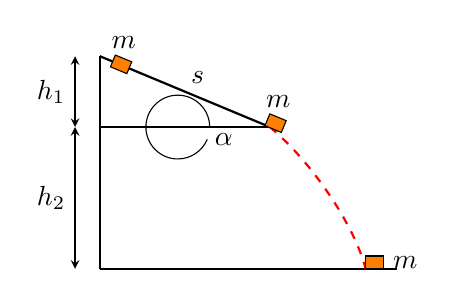
\begin{tikzpicture}[scale=0.9, >=stealth]

% Coordinates
\coordinate (A) at (0,3);
\coordinate (B) at (2.4,2);
\coordinate (C) at (0,2);
\coordinate (D) at (0,0);
\coordinate (E) at (4.2,0);

% Wall and ground
\draw[thick] (A) -- (D);
\draw[thick] (D) -- (E);

% Roof slope
\draw[thick] (A) -- (B);

% Horizontal reference line at roof edge
\draw[thick] (C) -- (B);

% Falling trajectory
\draw[red, dashed, thick] (B) .. controls (3.0,1.5) and (3.6,0.6) .. (3.75,0);

% Height h1
\draw[<->] (-0.35,3) -- (-0.35,2);
\node[left] at (-0.35,2.5) {$h_1$};

% Height h2
\draw[<->] (-0.35,2) -- (-0.35,0);
\node[left] at (-0.35,1) {$h_2$};

% Slope length s
\node[above right] at (1.15,2.48) {$s$};

% Angle alpha
\draw (1.55,2) arc[start angle=0,end angle=337.4,radius=0.45];
\node at (1.75,1.82) {$\alpha$};

% Stone at top
\begin{scope}[shift={(0.15,2.85)}, rotate=-22.6]
\draw[fill=orange] (0,0) rectangle (0.25,0.18);
\node[above] at (0.13,0.18) {$m$};
\end{scope}

% Stone leaving roof
\begin{scope}[shift={(2.33,2.02)}, rotate=-22.6]
\draw[fill=orange] (0,0) rectangle (0.25,0.18);
\node[above] at (0.13,0.18) {$m$};
\end{scope}

% Stone on ground
\draw[fill=orange] (3.75,0) rectangle (4.0,0.18);
\node[right] at (4.0,0.09) {$m$};

\end{tikzpicture}
\end{center}

\pagebreak
\begin{enumerate}

\item A stone with mass $m = 0.2\,\mathrm{kg}$ starts to slide from rest from the top edge of a roof, as shown in the figure. The roof is inclined at an angle $\alpha = 40^\circ$.

The following data are given:

$$g = 10\,\mathrm{m/s^2}, \qquad h_1 = 3\,\mathrm{m}, \qquad h_2 = 15\,\mathrm{m}.$$

\begin{enumerate}
\item[(a)] Assuming that the roof is frictionless, determine the magnitude of the velocity of the stone at the moment it reaches the ground.

\item[(b)] Determine the impact velocity if friction acts along the inclined roof and the coefficient of kinetic friction is $\mu = 0.4$.

Neglect air resistance.
\end{enumerate}

The total vertical height difference between the initial and final positions is

$$H = h_1 + h_2 = 3\,\mathrm{m} + 15\,\mathrm{m} = 18\,\mathrm{m}.$$

\item[(a)] \textbf{Frictionless motion:} Since there is no friction, mechanical energy is conserved. Initially, the stone is at rest, therefore its initial kinetic energy is zero. The conservation of mechanical energy gives

$$m g H + \frac{1}{2} m v_i^2 = m g h_f + \frac{1}{2} m v_f^2.$$

Because $v_i = 0\,\mathrm{m/s}$ and the ground level is chosen as $h_f = 0\,\mathrm{m}$, the equation becomes

$$m g H = \frac{1}{2} m v_f^2.$$

After cancelling the mass:

$$g H = \frac{1}{2} v_f^2.$$

\pagebreak
Solving for the final velocity:

$$v_f = \sqrt{2 g H}.$$

Substituting the numerical values:

$$v_f = \sqrt{2 g H} = \sqrt{2 \cdot 10\,\mathrm{m/s^2} \cdot 18\,\mathrm{m}}= 18.97\,\mathrm{m/s}.$$

\item[(b)] \textbf{Motion with friction:} In this case, friction performs negative work on the stone. The conservation of mechanical energy becomes

$$m g H = W_{\mathrm{fric}} + \frac{1}{2} m v_f^2.$$

The friction force is

$$F_{\mathrm{fric}} = \mu N = \mu m g \cos\alpha.$$

\pagebreak
The length of the inclined roof is

$$s = \frac{h_1}{\sin\alpha} = \frac{3\,\mathrm{m}}{\sin 40^\circ}.$$

The work done by friction is

$$W_{\mathrm{fric}} = F_{\mathrm{fric}} s = \mu m g \cos\alpha \cdot s.$$

Substituting this into the energy equation:

$$m g H = \mu m g \cos\alpha \cdot s + \frac{1}{2} m v_f^2.$$

After dividing by the mass and rearranging:

$$v_f = \sqrt{2 g H - 2 \mu g \cos\alpha \cdot s}.$$

\pagebreak
Substituting the numerical values:

$$v_f = \sqrt{2 \cdot 10\,\mathrm{m/s^2} \cdot 18\,\mathrm{m} - 2 \cdot 0.4 \cdot 10\,\mathrm{m/s^2} \cdot \cos 40^\circ \cdot \frac{3\,\mathrm{m}}{\sin 40^\circ}}= 18.20\,\mathrm{m/s}.$$

\end{enumerate}
 
\pagebreak
\item From a water reservoir, water flows to a turbine located 100.5\,m below. 2.8\,$m^3$ of water passes through the turbine per minute. The efficiency of the turbine is 80\%. Neglecting air resistance and the minimal kinetic energy of the water leaving the turbine, calculate the power output of the turbine! The density of water is 1000\,kg/$m^3$, g=9.8\,m/$s^2$.

\begin{center}
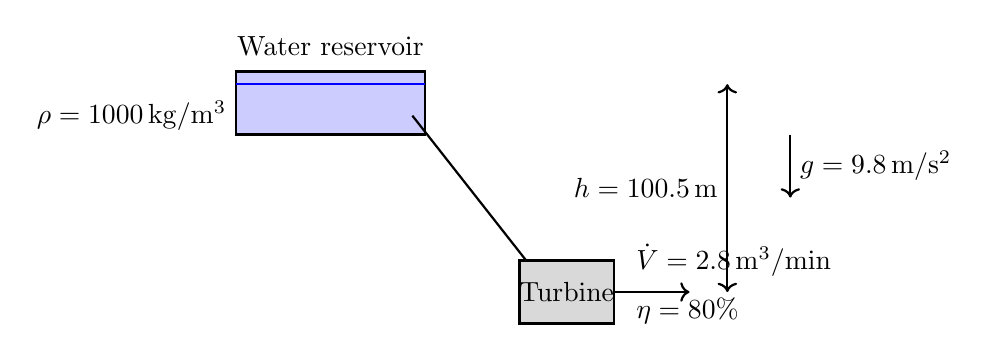
\begin{tikzpicture}[scale=0.8]

% reservoir
\fill[blue!20] (-3,4) rectangle (0,5);
\draw[thick] (-3,4) rectangle (0,5);

\node at (-1.5,5.4) {Water reservoir};

% water surface
\draw[blue, thick] (-3,4.8) -- (0,4.8);

% pipe
\draw[thick] (-0.2,4.3) -- (2,1.5);

% turbine
\draw[fill=gray!30, thick] (1.5,1) rectangle (3,2);

\node at (2.25,1.5) {Turbine};

% outgoing water
\draw[thick,->] (3,1.5) -- (4.2,1.5);

% height arrow
\draw[<->, thick] (4.8,4.8) -- (4.8,1.5);

\node[left] at (4.8,3.15) {$h = 100.5\,\mathrm{m}$};

% labels
\node[left] at (-3,4.3) {$\rho = 1000\,\mathrm{kg/m^3}$};

\node[right] at (3.2,2.0)
{
$\dot{V} = 2.8\,\mathrm{m^3/min}$
};

\node[right] at (3.2,1.2)
{
$\eta = 80\%$
};

% gravity arrow
\draw[->, thick] (5.8,4) -- (5.8,3);

\node[right] at (5.8,3.5)
{
$g = 9.8\,\mathrm{m/s^2}$
};

\end{tikzpicture}
\end{center}

%The given data are: $h = 100.5\,\mathrm{m}$, $V = 2.8\,\mathrm{m^3}$, $t = 1\,\mathrm{min} = 60\,\mathrm{s}$, $\eta = 80\% = 0.80$, $\rho = 1000\,\mathrm{kg/m^3}$, $g = 9.8\,\mathrm{m/s^2}$.

The water flowing from the reservoir loses gravitational potential energy. This potential energy is converted into mechanical energy at the turbine. Since the turbine is not ideal, only a fraction of this energy appears as useful output energy. The mass of the water passing through the turbine in one minute is calculated from the density and the volume:

\vskip -10 pt
$$m = \rho V.$$

Substituting the numerical values gives:

$$m =  \rho V = 1000\,\mathrm{kg/m^3} \cdot 2.8\,\mathrm{m^3} = 2800\,\mathrm{kg}.$$

The gravitational potential energy of this amount of water is:

$$E_{\mathrm{pot}} = mgh.$$

\pagebreak
Substituting the numerical values:
\vskip -10 pt
$$E_{\mathrm{pot}} =  mgh = 2800\,\mathrm{kg} \cdot 9.8\,\mathrm{m/s^2} \cdot 100.5\,\mathrm{m}.$$

Therefore,
\vskip -10 pt
$$E_{\mathrm{pot}} = 2757720\,\mathrm{J}.$$

The input power of the turbine is the potential energy delivered to the turbine per unit time:
\vskip -10 pt
$$P_{\mathrm{in}} = \frac{E_{\mathrm{pot}}}{t}.$$

Therefore,

$$P_{\mathrm{in}} = \frac{2757720\,\mathrm{J}}{60\,\mathrm{s}}.$$

\pagebreak
Hence the input power is:
\vskip -10 pt
$$P_{\mathrm{in}} = 45962\,\mathrm{W} \approx 46.0\,\mathrm{kW}.$$

The useful output power is obtained by multiplying the input power by the efficiency of the turbine:
\vskip -10 pt
$$P_{\mathrm{out}} = \eta P_{\mathrm{in}}.$$

Substituting the efficiency:
\vskip -10 pt
$$P_{\mathrm{out}} =  \eta P_{\mathrm{in}} = 0.80 \cdot 45962\,\mathrm{W} = 36770\,\mathrm{W} \approx 36.8\,\mathrm{kW}.$$

Therefore, the useful power output of the turbine is approximately

$$\boxed{P_{\mathrm{out}} = 36.8\,\mathrm{kW}.}$$

  
\pagebreak
\item A vehicle traveling with velocity $v$ on a horizontal road decelerates uniformly over a distance $s$. What slope angle $\alpha$ will keep the vehicle at rest in its braked state on a similarly graded road? Neglecting air resistance.

\begin{center}
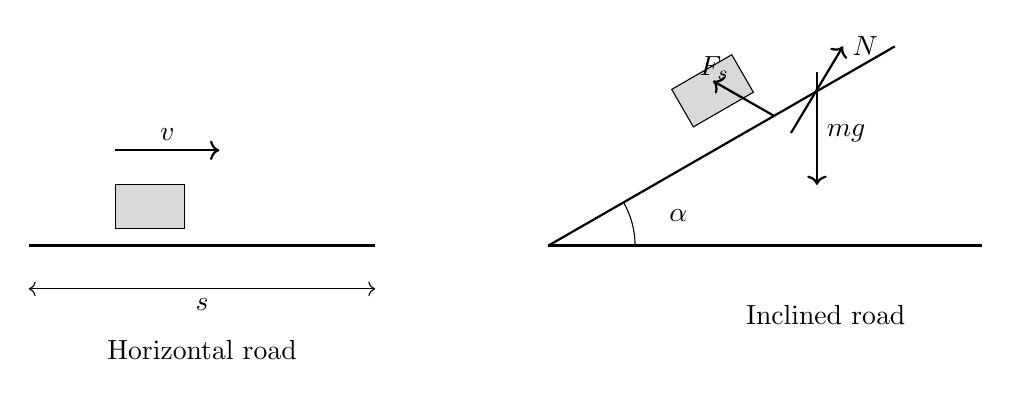
\begin{tikzpicture}[scale=1.1]

% horizontal road
\draw[thick] (-5,0) -- (-1,0);

% braking car
\draw[fill=gray!30] (-4,0.2) rectangle (-3.2,0.7);

% velocity arrow
\draw[->, thick] (-4,1.1) -- (-2.8,1.1);
\node[above] at (-3.4,1.1) {$v$};

% braking distance
\draw[<->] (-5,-0.5) -- (-1,-0.5);
\node[below] at (-3,-0.5) {$s$};

\node at (-3,-1.2) {Horizontal road};

% inclined plane
\draw[thick] (1,0) -- (6,0);
\draw[thick] (1,0) -- (5,2.3);

% parked car on slope
\begin{scope}[rotate=30]
\draw[fill=gray!30] (3.0,-0.15) rectangle (3.8,0.35);
\end{scope}

% angle alpha
\draw (2,0) arc (0:30:1);
\node at (2.5,0.35) {$\alpha$};

% gravity force
\draw[->, thick] (4.1,2.0) -- (4.1,0.7);
\node[right] at (4.1,1.3) {$mg$};

% friction force
\draw[->, thick] (3.6,1.5) -- (2.9,1.9);
\node[above left] at (3.2,1.8) {$F_s$};

% normal force
\draw[->, thick] (3.8,1.3) -- (4.4,2.3);
\node[right] at (4.4,2.3) {$N$};

\node at (4.2,-0.8) {Inclined road};

\end{tikzpicture}
\end{center}

\pagebreak
First, we determine the coefficient of static friction $\mu$ from the braking motion on the horizontal road. During braking, the vehicle moves with uniform deceleration. Its initial velocity is $v$, its final velocity is $0\,\mathrm{m/s}$, and the braking distance is $s$. The maximum braking force is provided by the static friction force between the tires and the road. On a horizontal road, the normal force is $N = mg$, therefore the maximum static friction force is
\vskip -10 pt
$$F_s = \mu N = \mu mg.$$

According to Newton's second law, this force causes the deceleration of the vehicle:
\vskip -10 pt
$$ma = \mu mg.$$

After cancelling the mass $m$, we obtain
\vskip -10 pt
$$a = \mu g.$$

\pagebreak
The uniformly decelerated motion can also be described by the kinematic relation
\vskip -10 pt
$$v_f^2 = v_i^2 - 2as.$$

Here the final velocity is $v_f = 0\,\mathrm{m/s}$ and the initial velocity is $v_i = v$, therefore
\vskip -10 pt
$$0 = v^2 - 2as.$$

Solving this equation for the magnitude of the deceleration gives
\vskip -10 pt
$$a = \frac{v^2}{2s}.$$

Since the same deceleration is produced by the maximum static friction force, we can equate the two expressions for $a$:

$$\mu g = \frac{v^2}{2s}.$$

\pagebreak
Therefore, the coefficient of static friction is
\vskip -10 pt
$$\mu = \frac{v^2}{2gs}.$$

Now consider the same fully braked vehicle on an inclined road with slope angle $\alpha$. The component of the gravitational force parallel to the slope is
\vskip -10 pt
$$mg\sin\alpha.$$

The normal force perpendicular to the slope is
\vskip -10 pt
$$N = mg\cos\alpha.$$

The maximum static friction force is therefore
\vskip -10 pt
$$F_s = \mu N = \mu mg\cos\alpha.$$

\pagebreak
For the vehicle to remain at rest on the slope, the downslope component of gravity must be balanced by the static friction force:
\vskip -10 pt
$$mg\sin\alpha = \mu mg\cos\alpha.$$

After cancelling $mg$, we get
\vskip -10 pt
$$\sin\alpha = \mu\cos\alpha.$$

Dividing both sides by $\cos\alpha$ gives
\vskip -10 pt
$$\tan\alpha = \mu.$$

Therefore, the slope angle is
\vskip -10 pt
$$\alpha = \arctan\mu.$$

\pagebreak
Substituting the expression for $\mu$ obtained from the braking distance:
$$\alpha = \arctan\left(\frac{v^2}{2gs}\right).$$

Hence, the required slope angle is
$$\boxed{\alpha = \arctan\left(\frac{v^2}{2gs}\right)}.$$
\end{enumerate}

\end{frame}

% ----------------------------------------------------------------------------------------------------------------------------------------

\begin{frame}[fragile,squeeze,allowframebreaks]
\frametitle{Wave Optics}

\begin{enumerate}

\item The wave shown in the figure was generated by a $60\,\mathrm{Hz}$ resonator. Determine:
\begin{enumerate}
\item[a)] amplitude of the wave
\item[b)] frequency of the wave
\item[c)] wavelength of the wave
\item[d)] propagation speed of the wave
\item[e)] period of the wave
\end{enumerate}

\begin{center}
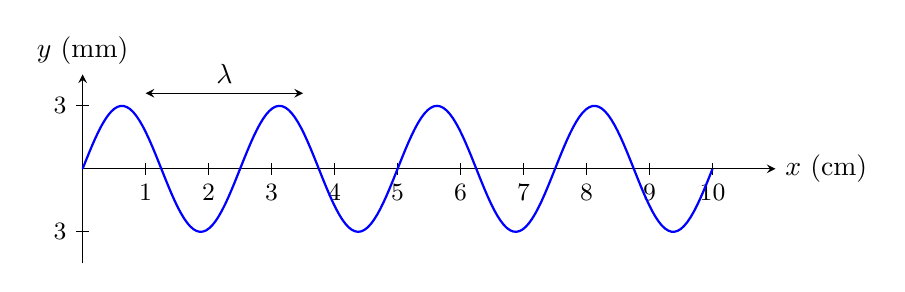
\begin{tikzpicture}[scale=0.8, >=stealth]

\draw[->] (0,0) -- (11,0) node[right] {$x\ (\mathrm{cm})$};
\draw[->] (0,-1.5) -- (0,1.5) node[above] {$y\ (\mathrm{mm})$};

\foreach \x in {1,2,...,10}
    \draw (\x,0.1) -- (\x,-0.1) node[below] {\small \x};

\foreach \y in {-1,1}
    \draw (0.1,\y) -- (-0.1,\y) node[left] {\small 3};

\draw[thick, blue, domain=0:10, samples=200]
    plot (\x, {1*sin(deg(2*pi*\x/2.5))});

\draw[<->] (1,1.2) -- (3.5,1.2);
\node[above] at (2.25,1.2) {$\lambda$};

\end{tikzpicture}
\end{center}

\begin{eqnarray*}
A &=& 3 \cdot 10^{-3}\,\mathrm{m} \\
f &=& 60\,\mathrm{Hz}\\
\lambda &=& 2.5\,\mathrm{cm} = 0.025\,\mathrm{m}\\
v &=& f \lambda = 1.5\,\mathrm{m/s}\\
T &=& \frac{1}{f} = 0.0167\ \mathrm{s}
\end{eqnarray*}

\pagebreak

\item A wave propagating along a string can be defined as follows (with x in meters, t in seconds): $y = 0.02\,m \sin(30t - 4x).$ Determine the:
\begin{enumerate}
\item[a)] amplitude
\item[b)] frequency
\item[c)] speed
\item[d)] wavelength
\end{enumerate}
\vskip -40 pt
\begin{eqnarray*}
A &=& 0.02\,\mathrm{m}\\  
\omega &=& 30\,\mathrm{rad/s}\\  
k &=& 4\,\mathrm{rad/m}\\  
f &=& \frac{\omega}{2\pi} = 4.77\,\mathrm{Hz}\\ 
v &=& \frac{\omega}{k} = 7.5\,\mathrm{m/s}\\  
\lambda &=& \frac{2\pi}{k} = 1.57\,\mathrm{m}  
\end{eqnarray*}


\pagebreak

\item Consider a wave given by the equation$f(x,t) = A e^{-B(x-vt)^2}.$ Prove that this wave equation satisfies the general one-dimensional wave equation.

\medskip
  
Substitute $u = x - vt$, then both second derivatives give the same structure, hence wave equation satisfied.

\pagebreak

\item Determine the amplitude, frequency, and wavelength of the wave shown in the figure below, if the propagation speed of the wave is 300\,m/s. Write a solution for the wave if at t=0\,s the wave appears as shown in the figure.

\begin{center}
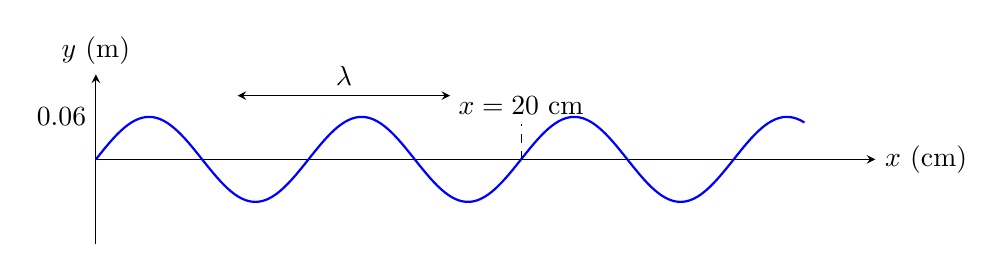
\begin{tikzpicture}[scale=0.9, >=stealth]

\draw[->] (0,0) -- (11,0) node[right] {$x\ (\mathrm{cm})$};
\draw[->] (0,-1.2) -- (0,1.2) node[above] {$y\ (\mathrm{m})$};

\draw[thick, blue, domain=0:10, samples=200]
    plot (\x, {0.6*sin(deg(2*pi*\x/3))});

\node[left] at (0,0.6) {$0.06$};

\draw[<->] (2,0.9) -- (5,0.9);
\node[above] at (3.5,0.9) {$\lambda$};

\draw[dashed] (6,0) -- (6,0.5);
\node[above] at (6,0.5) {$x=20\ \mathrm{cm}$};

\end{tikzpicture}
\end{center}

\begin{eqnarray*}
A &=& 0.06\,\mathrm{m}\\  
\lambda &=& 0.03\,\mathrm{m}\\  
f &=& \frac{v}{\lambda} = 10000\,\mathrm{Hz}\\
\omega &=& 2\pi f\\  
k &=& \frac{2\pi}{\lambda}  
\end{eqnarray*}
  
Wave:  

$$y(x,t) = 0.06 \sin(kx - \omega t)$$

\pagebreak

\item For a wave propagating along a string with a frequency of 30\,Hz, $\lambda$ = 60\,cm, A = 2\,mm, write the solution in SI units.

\begin{eqnarray*}
\omega &=& 60\pi\,\mathrm{rad/s}\\
k &=& \frac{2\pi}{0.6}\\  
y(x,t) &=& 2 \cdot 10^{-3} \sin(kx - \omega t)
\end{eqnarray*}  

\pagebreak

\item A wave solution is given by $y = 0.27 \sin(12x - 500t)\,mm$, where x is in meters and t is in seconds. For the transverse wave at x=20\,cm, determine:
\begin{enumerate}
\item[a)] its speed
\item[b)] its acceleration
\item[c)] What is the displacement of the point at t=4\,s?
\end{enumerate}

\begin{eqnarray*}
A &=& 2.7 \cdot 10^{-4}\,\mathrm{m} \\  
v &=& \frac{500}{12} = 41.67\,\mathrm{m/s} \\ 
v(t) &=& -0.135 \cos(2.4 - 500t)\,\mathrm{m/s} \\ 
a(t) &=& -67.5 \sin(2.4 - 500t)\,\mathrm{m/s^2}\\  
y(4) &\approx& 2.6 \cdot 10^{-4}\,\mathrm{m}
\end{eqnarray*}  

\end{enumerate}

\end{frame}

% ----------------------------------------------------------------------------------------------------------------------------------------

\begin{frame}
%\frametitle{Minden jó, ha a vége jó}

\vfill
\begin{center}
\textbf{\huge The End}

\bigskip
Thank you for your attention!
\end{center}
\vfill
%\textbf{Acknowledgements} Thank you for the course materials for Szilárd~ZSÓKA and Zoltán~VARGA.
\end{frame}

\end{document}


% ++++++++++++++++++++++++++++++++++++++++++++++++++++++++++++++++++++++++++++++++++++++++++++++++++++++++++++++++++++++++++++++++++++


%%%%%%%%%%%%%%%%%%%%%%%%%%%%%%%%%%%%%%%%%%%%%%%%%%%%%%%%%%%%


\section*{5. Exercise}

Let:

\[
f(\omega t \pm kx + \phi)
\]

be an arbitrary twice differentiable continuous function.

Prove that it satisfies the one-dimensional wave equation.

\subsection*{Solution}



%%%%%%%%%%%%%%%%%%%%%%%%%%%%%%%%%%%%%%%%%%%%%%%%%%%%%%%%%%%%

\section*{6. Exercise}

The displacement of a transverse wave is:

\[
y(x,t)=0.27\sin(12x-500t)\ \mathrm{mm}
\]

where \(x\) is measured in meters and \(t\) in seconds.

At the point \(x=0.2\ \mathrm{m}\), determine:

\begin{enumerate}[label=\alph*)]
\item the velocity,
\item the acceleration,
\item the displacement at \(t=4\ \mathrm{s}\).
\end{enumerate}

\subsection*{Solution}



\end{document}